\documentclass{cslthse-msc}
\usepackage[utf8]{inputenc}
\usepackage[english]{babel}
%\usepackage[T1]{fontenc}
\usepackage{graphicx}
\usepackage{amsfonts}
\usepackage{amssymb}
\usepackage{amsmath}
\usepackage[titletoc, header, page]{appendix}
\usepackage{amsthm}
\usepackage{float}
\restylefloat{table}
\usepackage[hidelinks]{hyperref}
\usepackage{multicol}
\usepackage{wasysym}
\usepackage[square,sort,comma,numbers]{natbib}
\usepackage{pgfplots}
\pgfplotsset{compat=1.3}
\pgfplotsset{major grid style={color=black!50, thick}}
\pgfplotsset{every axis legend/.append style={fill=none, draw=none}}
\usepackage{tikz}
\usetikzlibrary{positioning}
\usepackage{fancyvrb}
\fvset{tabsize=3}
\fvset{fontsize=\small}
\usepackage{pdfpages}
\usepackage{enumerate}
\newcommand{\code}{\texttt}
\newcommand{\density}{dE}
\newtheorem{lemma}{Lemma}

\title{\huge{Algorithmic Engineering Aspects of Fast Zeta Transform-based Graph Colouring Algorithms}}

\author{Mats Rydberg \\
    {\normalsize \href{mailto:rydbergmats@gmail.com}{\texttt{rydbergmats@gmail.com}}}}
\supervisor{Thore Husfeldt, \href{mailto:thore.husfeldt@cs.lth.se}{\code{thore.husfeldt@cs.lth.se}}}
\examiner{Jonas Skeppstedt, \href{mailto:thore.husfeldt@cs.lth.se}{\code{jonas.skeppstedt@cs.lth.se}}}
\date{\today}

\acknowledgements{
Thank you.
}

\theabstract{
The \emph{chromatic polynomial} $\chi_G(t)$ of a graph $G$ on $n$ vertices is a univariate polynomial of degree $n$, passing through the points $(q, P(G,q))$ where $P(G,q)$ is the number of $q$-colourings of $G$. In this paper, we present an implementation of an algorithm by Björklund, Husfeldt, Kaski and Koivisto that computes $\chi_G(t)$ in time $O^*(2^n)$ and space $O^*(1.2916^n)$. We compare the performance of two different core libraries to eachother and show our performance against an implementation done by Haggard, Pearce and Royle from 2010. 
We also present the chromatic polynomials for a small Queen graph and a certain graph specified by Hillar and Windfeldt.
}

\keywords{graph colouring, algorithms, chromatic polynomial, master's thesis, parallelization}

\begin{document}
\makefrontmatter

\chapter{Introduction}
In this report, we will present experimental results from simulations and tests run on implementations of a few algorithms presented in a report by Björklund, Husfeldt, Kaski and Koivisto \cite{cov_pack}. The two main results of that report is an algorithm for performing an algorithm, \emph{the fast zeta transform}, with reduced space requirement from before, along with an application of this result on an algorithm for computing the \emph{chromatic polynomial} of a graph. Our focus will lie on the chromatic polynomial algorithm, but in the process of constructing that program, we also completed implementations of three more direct applications of the fast zeta transform algorithm, solving the familiar \emph{set cover}, \emph{set partition} and \emph{set packing} problems.

\section{Report structure}
We will begin with a theoretical introduction into the area of graph theory, present some previous scientific results, continue with the problem statement that has guided our work during this Master's Thesis, and then shortly mention some of our main results. In the following chapters, we will go through the working process in a more detailed manner, present reflections and in-depth results from the experiments that we have carried through. In the appendix we present selected parts of the code base which make up our implementations, and the chromatic polynomials of a few mentioned graphs.

\section{Preliminaries}
Here we present all necessary definitions and theoretical notation that will be used in this report. In the case of a ill-defined variable used in the following, we refer the reader to this section.

\subsection{Set problems} \label{setproblems}
In the \emph{set cover} problem, we are given a set $U$, a family $\mathcal{F}$ of subsets of $U$ and a natural number $q$, and are tasked with the problem of deciding whether there are $q$ sets in $\mathcal{F}$ whose union equals $U$. In the \emph{set partition} problem, we must decide whether there are $q$ \emph{pairwise disjoint} sets in $\mathcal{F}$ whose union equals $U$. In the \emph{set packing} problem, we must decide whether there are $q$ pairwise disjoint subsets of $\mathcal{F}$ whose union is a \emph{subset} of $U$. Two sets are disjoint if they have no elements in common.

The \emph{counting} versions of these problems asks instead \emph{how many} distinct such selections of sets that exist. In this report, we will only discuss counting versions of these (and other) problems.

\subsection{Chromatic polynomial}
A \emph{graph} is a set of two distinct abstract units called \emph{vertices} and \emph{edges}; an edge being a connection between two vertices. The vertices are contained in a vertex set $V$, and we say that the graph has \emph{order} $n$ if $|V| = n$. Similarly, we have an edge set $E$, and say that the graph has \emph{size} $m = |E|$; the maximum size of a graph of order $n$ is $\binom{n}{2} = n(n-1)/2$. We write a graph $G$ as $G = (V,E)$. An edge $vw \in E$ implies $v \in V$ and $w \in V$, where $v$ and $w$ are the vertices connected by $vw$; $v$ and $w$ are said to be \emph{adjacent}. In this report, edges are undirected, have multiplicity $leq 1$ and are never loops. An example graph is found in figure~\ref{moser}.

In the \emph{graph colouring} problem, we are given a graph $G = (V,E)$ and a natural number $q$, and tasked to determine whether there exists a mapping $\sigma: V \rightarrow [q]$ where $[q] = \{0,1,\ldots,q\}$, such that $\sigma(v) \neq \sigma(w)$ for each $vw \in E$. In other words, $\sigma$ is an assignment of one of $q$ \emph{colours} to each vertex such that no two adjacent vertices get the same colour; we call such an assignment a \emph{proper $q$-colouring} of $G$. The counting version of this problem asks \emph{how many} distinct such mappings exist; we call this number $P(G,q)$.

The \emph{chromatic polynomial} $\chi_G(t)$ of the graph $G$ is the polynomial of degree $n$ in one indeterminate that passes through each point $(q, P(G,q))$. To determine $\chi_G(t)$, by for example specifying its coefficients, it suffices to determine the numbers $P(G,q)$ for each $q \leq n$ and then construct $\chi_G(t)$ by interpolation, as $n + 1$ points uniquely identifies an $n$-degree polynomial. Four characteristics of any chromatic polynomial is that the coefficient of $t^n$ is always one, the coefficient of $t^{n-1}$ is always $-m$, the coefficient of $t^0$ is always 0, and the signs of the coefficients are alternating positive and negative. Figure~\ref{moser} presents an example graph and its chromatic polynomial.

 \begin{figure}[bt]
 \centering
 \begin{multicols}{2}
 \begin {tikzpicture}[-latex ,auto ,on grid ,semithick , inner sep = 2,
a/.style ={ circle, draw, text=white, minimum width = 3 mm, fill = black },
b/.style ={ circle, draw, text=black, minimum width = 3 mm, fill = black!66 },
c/.style ={ circle, draw, text=black, minimum width = 3 mm, fill = black!33 },
d/.style ={ circle, draw, text=black, minimum width = 3 mm, fill = black!0 }]
\node[a] (1) at (-3,-3) {$1$};
\node[b] (2) at (-2,-1) {$2$}
  edge [-] (1);
\node[c] (3) at (-1,-2) {$3$}
  edge [-] (1)
  edge [-] (2);
\node[a] (4) at (0,0) {$4$}
  edge [-] (2)
  edge [-] (3);
\node[c] (5) at (1,-2) {$5$}
  edge [-] (4);
\node[b] (6) at (2,-1) {$6$}
  edge [-] (4)
  edge [-] (5);
\node[d] (7) at (3,-3) {$7$}
  edge [-] (1)
  edge [-] (5)
  edge [-] (6);
\end{tikzpicture}

\columnbreak

\begin{tabular}{ll}
$\chi_{MS}(t) = $ & $t^7 - 11t^6 + 51t^5 $ \\
& $- 129t^4 + 188t^3$ \\
& $- 148t^2 + 48t $ \\
& \\
$\chi_{MS}(4) = $ & $ 384 $ \\
\end{tabular}

\end{multicols}
  \caption{To the left, the Moser Spindle graph, $MS$, on $n = 7$ vertices and $m = 11$ edges, coloured in four different gray scales. To the right, its chromatic polynomial $\chi_{MS}(t)$.}
  \label{moser}
\end{figure}

\subsection{Miscellaneous}
The \emph{chromatic number} $\chi(G)$ of the graph $G$ is the smallest $q$ for which $\chi_G(q) \neq 0$; it is the minimum amount of colours needed to produce a proper colouring of $G$. Graph \emph{density} $\density{}$ is the size of the graph over its maximum size.

\section{Previous work}
Present some history, present fastest for 3 colours, 4 colours, fastest general colouring, naive colouring, etc. Fastest count for 3 colours, 4 colours, etc.

%TODO


The chromatic polynomial was specified in 1912 by Birkhoff \cite{birkhoff}, who defined it for planar graphs with the intent on proving the Four Colour Theorem. Whitney extended its definition to general graphs in 1932 \cite{whitney}, and Tutte incorporated it into what is now known as the Tutte polynomial. See for example Ellis-Monaghan and Merino \cite{tuttebook} for more in-depth analysis of the Tutte polynomial.

The most commonly referenced problem in the field of graph colouring is the one of producing an \emph{optimal} colouring of a given graph, that is, a colouring using $\chi(G)$ colours. Trivially, this can of course be done by exhaustively searching through all possible assignments of the $n$ vertices to $q$ colours, starting from $q = 3$ and moving upwards (since 2-colouring is a problem in P), each step taking time $O^*(q^n)$, bound at the last step by $O^*(n^n)$. 

For general colouring, Christofides~\cite{christo} constructed the first non-trivial algorithm in 1971, running in time $O(n!)$, a result which was first improved by Lawler~\cite{lawler} in 1976, 

Beigel and Eppstein~\cite{3coloring} currently hold the record of 3-colouring since 2005, which takes them $O^*(1.3289^n)$ time; considerably better than the naive $O^*(3^n)$. To achieve this bound, they use a reduction of the colouring into a constraint satisfactory problem, in which they are able to find divisions of the problem into smaller subproblems, and solving these individually.
Fomin, Gaspers and Saurabh~\cite{4coloring} invented the best known algorithm for 4-colouring in 2007, running in $O^*(1.7272^n)$ time. They base their algorithm on the proof that a graph will either allow efficient branching procedures to reduce the size of the problem, or it will have a small pathwidth, allowing for efficient algorithms to exploit its path decomposition.

In 2010, Haggard, Pearce and Royle \cite{haggard} published a program, referred to in the following as \textbf{HPR}, to compute the Tutte polynomial for graphs using a deletion-contraction algorithm. HPR exploits the isomorphism of induced subgraphs to obtain good performance, and can easily handle many instances of non-trivial sizes. Using the fact that the Tutte polynomial encodes the chromatic polynomial (as well as other graph invariants), HPR is also designed to output $\chi_G(t)$. 
In 2011, Björklund, Husfeldt, Kaski and Koivisto \cite{cov_pack} presented an algorithm to compute the chromatic polynomial in time $O^*(2^n)$ and space $O^*(1.2916^n)$, referred to here as the \textbf{BHKK} algorithm. The notation $O^*$ hides polylogarithmic factors.

\section{Problem statement}
The main question is whether the BHKK algorithm performs well in practice. Irrefutably, it does provide theoretical improvements in the form of a better asymptotic bound on space usage. Intuitively, using less memory means we spend less time handling the memory, and this could reduce also the time consumption. But as the asymptotic bound stays solid, we can not know for sure how impactful such a reduction could be. Björklund \emph{et al} also mentions that BHKK parallelizes well, and provides theoretical bounds suggesting how much of an improvement parallelization provides \cite[p.10]{cov_pack}. Haggard \emph{et al} does not perform an asymptotic analysis of their algorithm, but simply shows experimental results showing it performs ``well''. We will use HPR as a reference in our experiments, making us able to conclude that BHKK does provide improvement if it outperforms HPR. We attempt to answer the following direct questions:

\begin{enumerate}
 \item Does BHKK outperform HPR as the order of the graph increases? \label{ngrow}
 \item What is the maximum order of a graph that BHKK can compute the chromatic polynomial in human time for? \label{maxn}
 \subitem With ``human time'', we mean less than a month.
 \item How does the graph size affect HPR and BHKK, respectively? \label{mgrow}
 \item How much of an improvement can parallelization provide in practice? \label{parallel}
\end{enumerate}

\section{Main results}
The answers to the stated questions are, in short:

\begin{enumerate}
 \item Yes, for $n > 21$.
 \item 30.
 \item BHKK is faster with increasing size; HPR is slower.
 \item About 600\%.
\end{enumerate}

We find proof that BHKK does provide better asymptotic behaviour than HPR, for random graphs of quadratic size. We were able to compute the chromatic polynomial of a 30-order graph, but were unable to compute it for a 36-order graph.

\chapter{Approach}
In this chapter we present an in-depth view of the algorithms studied, including special characteristics that aided us in their implementation. We describe the implementation process in some detail and present the external libraries that were employed. Finally we describe the setup of the experimental environment, including our measurement methods.


\section{Studied algorithms}
While our emphasis lies on the BHKK algorithm for computing chromatic polynomials, we will here briefly describe also a few other algorithms that were studied as a part of our work.

\subsection{The fast zeta transform}
Björklund \emph{et al} \cite{cov_pack} base their work on an improvement of the fast zeta transform, FZT. There are two versions of FZT, the down-zeta transform $f\zeta$ and the up-zeta transform $f'\zeta$, and they are defined as
\[
 f\zeta(X) = \sum_{Y \subseteq X} f(Y), \qquad f'\zeta(X) = \sum_{Y \supseteq X} f(Y)
\]
for a function $f$ defined for subsets $X$ of an $n$-sized universe $U$. In \cite[p.5]{cov_pack} is described pseudo-code for an algorithm computing the fast zeta transform in time and space exponential in $n$. 

In the \emph{linear-space} fast zeta transform, we are given additional input in the form of a set family $\mathcal{F}$ that contains all defined inputs for the function $f$. In other words, $f(X) = 0$ if $X \notin \mathcal{F}$. The main idea is to split $U$ into disjoint parts $U_1$ and $U_2$ with sizes $n_1$ and $n_2$ respectively, and to iterate over them separately. The algorithm is outlined in \cite[sec.3]{cov_pack}, and uses $O^*(|\mathcal{F}|)$ space:

\begin{enumerate}[1.]
 \item For each $X_1 \in U_1$ do:
 \begin{enumerate}[a)]
  \item For each $Y_2 \in U_2$, set $g(Y_2) \leftarrow 0$.
  \item For each $Y \in \mathcal{F}$, if $Y \cap U_1 \subseteq X_1$ then set $g(Y \cap U_2) \leftarrow g(Y \cap U_2) + f(Y)$.
  \item Compute $h \leftarrow g\zeta$.
  \item For each $X_2 \subseteq U_2$, output $h(X_2)$ as the value $f\zeta(X_1 \cup X_2)$. \label{fztoutput}
 \end{enumerate}
\end{enumerate}
With $n_2 = |\mathcal{F}|$, the linear-space bound is guaranteed.

\subsection{Coverings, partitionings and packings}
The linear-space FZT has direct applications on some set problems, see section~\ref{setproblems}. For $q$-cover, the function $f$ is $f(Y) = [ Y \in \mathcal{F} ]$, where $[P]$ denotes one if $P$ is true, and zero otherwise, and we find the number of $q$-covers as 
\begin{equation} \label{cq}
c_q(\mathcal{F}) = \sum_{X \in U} (-1)^{|U \setminus X|} f\zeta(X)^q.
\end{equation}
In the algorithm, we in step~\ref{fztoutput} do not output the values $h(X_2)$, but sum them according to \ref{cq}, outputting the resulting value $c_q$.

The number of $q$-partitions is the $n$th coefficient of the polynomial $d_q$, derived as in \ref{cq}, but with $f = [Y \in \mathcal{F}]z^{|Y|}$ operating in a ring of polynomials, with indeterminate $z$, instead. Now we perform all arithmetics using polynomials instead of integers, a fact we will see having a substantial impact on time and space requirements.

Finally, for $q$-packings, 


\subsection{Chromatic polynomial}
By adapting the linear-space FZT, an algorithm for the chromatic polynomial was designed in \cite{cov_pack}. The space bound for the resulting algorithm is increased to $O^*(1.29153^n)$.

Our input is an undirected graph $G$ on $n$ vertices with $m$ edges. The main subroutine counts the number of ways to colour $G$ using $q$ colours. This is done for $q = 0, 1, \ldots n$, yielding $n + 1$ points $(x_i, y_i)$. Interpolating on these points yields the chromatic polynomial $\chi_G(t)$.

The general idea of the algorithm uses the principle of inclusion-exclusion to count the proper $q$-colourings of $G$ by actually counting the number of ordered partitions of $V$ into $q$ \emph{independent sets}. The low space bound is obtained by splitting $V$ into two disjoint sets $V_1$ and $V_2$ of sizes $n_1$ and $n_2$ respectively, where $n_1 = \lceil n \frac{\log2}{\log3} \rceil$ and $n_2 = n - n_1$, and then run iterations of subsets of $V_1$ and store values dependent on (subsets of) $V_2$ \cite[sec. 5]{cov_pack}. 

The full algorithm in pseudo-code as follows:

\begin{enumerate}[{Step} A.]
\item \label{q} For $q = 0, 1, \ldots, n$, do
\begin{enumerate}[1.]
  \item Partition $V$ into $V_1$ and $V_2$ of sizes $n_1$ and $n_2$.
  \item \label{step1} For each $X_1 \subseteq V_1$, do
  \begin{enumerate}[a)]
  \item \label{indep1} For each independent $Y_1 \subseteq X_1$, do
\[ h[V_2 \setminus N(Y_1)] \leftarrow h[V_2 \setminus N(Y_1)] + z^{|Y_1|} \]
  \item \label{indep2} For each independent $Y_2 \subseteq V_2$, do
\[ l[Y_2] \leftarrow z^{|Y_2|} \]
  \item \label{multi} $h \leftarrow (h\zeta')\cdot l$
  \item $h \leftarrow h\zeta$
  \item \label{rstep}For each $X_2 \subseteq V_2$, do
\[ r \leftarrow r + (-1)^{n - |X_1| - |X_2|}\cdot h[X_2]^q \]
  \end{enumerate}
  \item Return coefficient $c_n$ of $z^n$ in $r$.
\end{enumerate}
\item Construct interpolating polynomial $\chi_G(t)$ on points $(q, c_{nq})$.
\item Return $\chi_G(t)$.
\end{enumerate}
Here, $N(Y)$ is the set of all vertices in $G$ adjacent to at least one vertex in $Y$. The arrays $h$ and $l$ of size $2^{n_2}$ contain polynomials (initialized to zeroes), $r$ is a polynomial. For a more detailed description, see \cite[p 9]{cov_pack}.

In subsequent sections, we will refer to this algorithm as ``the algorithm'', ``the BHKK algorithm'', or simply ``BHKK''.

\subsection{Optimizations}\label{optimizations}
Here are presented some improvements to the algorithm that are either natural, mentioned in \cite{cov_pack}, or invented by the author. This list is by no means exhaustive, nor is every item critical, but the ones we've explored proved to be efficient. 

\paragraph{Exploiting $q$}
First, we can consider optimizing on the basis of the value of $q$.
\begin{itemize}
\item For $q = 0$, there are 0 colourings, as no graph can be 0-coloured.
\item For $q = 1$, there are 0 colourings if and only if $|E| > 0$, otherwise there is exactly 1 colouring. This takes $O(n^2)$ time to check.
\item For $q = 2$, it is well-known that the graph can be coloured (or found to be non-colourable) in polynomial time using standard techniques (such as breadth-first search).
\end{itemize}

These optimizations will reduce the iterations of the loop at step \ref{q} by three.

\paragraph{Using $\omega_{min}(G)$}
A more sophisticated type of optimization involves exploiting the clique number $\omega(G)$, which is a lower bound on the chromatic number $\chi(G)$. Knowing that $\omega(G) \geq a$ for some constant $a$ would allow us to immediately skip all steps~\ref{q} where $q < a$. If $a = n$, we have the complete graph $K_n$, for which $\chi_G(t)$ is known.

Here we define the \emph{density} of a graph $G$ as $dE = m/\binom{n}{2}$, where $m$ is the number of edges in $G$. This immediately tells us the \emph{smallest possible} $\omega(G)$. Let us call it $\omega_{min}(G)$. In fact, the following holds:

\begin{lemma}\label{lemma1}
The number $\omega_{min}(G)$ is the lower bound of $\omega(G)$, and its value is
\[
\omega_{min}(G) = 
\begin{cases}
	  n - \binom{n}{2} + m & \text{if } m \geq \binom{n}{2} - \lfloor n/2 \rfloor \\
	  \lceil n / 2 \rceil - a & \text{if }  \lfloor n / 2 \rfloor \cdot \lceil n / 2 \rceil < m = \binom{n}{2} - a \lfloor n/2 \rfloor, a \in \mathbb{N}_+ \\
	  2 & \text{if } 0 < m \leq \lfloor n / 2 \rfloor \cdot \lceil n / 2 \rceil \\
	  1 & \text{if } m = 0 \\
\end{cases}
\]
\end{lemma}

% The idea of the proof is to add as many edges as possible to the empty graph $N_n$ without increasing $w(G)$, where $G$ is the resulting graph from adding edges.

\begin{proof}
 Trivially, $w(N_n) = 1$. This proves the lower-most bound.
 
 Next, consider the complete bipartite graph $K_{\alpha,\beta}$ on $n$ vertices; it is the graph with the most edges that has clique number 2. It is well-known that it has $\alpha \beta$ edges. To maximize this product, we make a half-half partition, setting $\alpha = \lfloor n / 2 \rfloor$ and $\beta = \lceil n / 2 \rceil$, giving $\alpha \beta = \lfloor n / 2 \rfloor \lceil n / 2 \rceil$. The point made is that there is no way of assigning more edges than this without yielding a higher clique number.
 
 Third, consider the complete graph $K_n$, with $w(K_n) = n$. Deleting an edge $vw$ will clearly reduce the clique number. Consider the subgraph $K \setminus \{v\}$; it has clique number $n - 1$. Removing an edge $uu', u \neq w, u' \neq w$ will lower clique number again by 1. This process may be repeated $\lfloor n / 2 \rfloor$ times. The resulting graph has $\binom{n}{2} - \lfloor n/2 \rfloor$ edges and clique number $n - \lfloor n/2 \rfloor$. This, together with the fact that removing one edge can lower clique number by maximum one, proves the uppermost bound. 
\end{proof}
For the final case, for which we do not provide a full proof, we observe that $\binom{n}{2} - \lfloor n/2 \rfloor - \lfloor n / 2 \rfloor \cdot \lceil n / 2 \rceil$ is a multiple of $\lfloor n/2 \rfloor$ (this is the variable $a$ in the lemma). It can be shown that this corresponds to the requirement of removing $\lfloor n/2 \rfloor$ edges to reduce clique number by one.

As we can see from Lemma~\ref{lemma1}, only graphs with $m > \lfloor n / 2 \rfloor \cdot \lceil n / 2 \rceil$ provides $\omega_{min}(G) > 2$ and for $q \leq 2$ we already have good optimizations. So how dense is a graph where this bound on $m$ holds? Let us specify the threshold density $T_{dE}(n)$ as

\[
T_{dE}(n) = 2\frac{\lfloor n / 2 \rfloor \cdot \lceil n / 2 \rceil}{n(n-1)} =
\begin{cases}
	  \frac{1}{2}n(n-1)^{-1} & \text{if } n \text{ even}\\
	  \frac{1}{2}(n+1)n^{-1} = T_{dE}(n+1) & \text{if } n \text{ odd}\\
\end{cases}
\]

In conclusion, any graph with $dE > T_{dE}(n)$ can optimize away at least one additional computation of step~\ref{q} above. It also follows that as $n \rightarrow \infty$ we will have $T_{dE}(n) \rightarrow \frac{1}{2}$. The following plot shows how fast we converge for graphs of sizes relevant for this paper.

\begin{center}
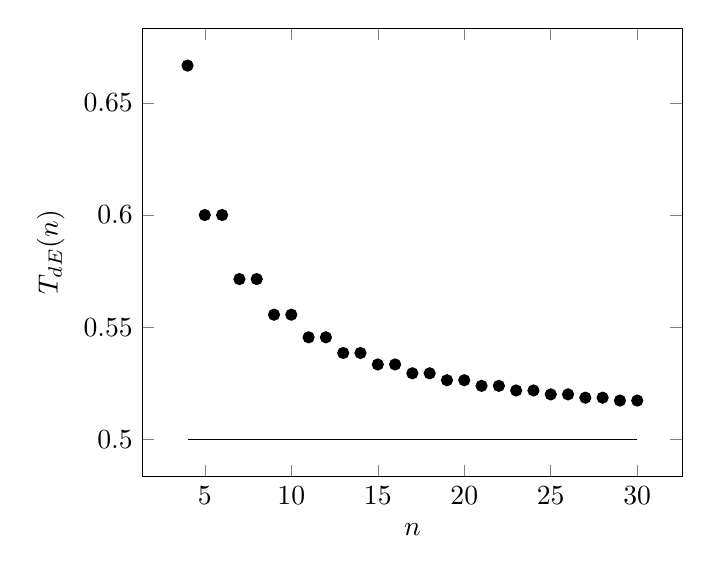
\begin{tikzpicture}
\begin{axis}[%samples at={4,5,6,7,8,9,10,11,12,13,14,...,23},
xlabel=$n$,
ylabel=$T_{dE}(n)$]
%\addplot[black, mark=*, samples=20, domain=4:23] {(2*floor((x/2)^2))/(x*(x-1))};
\addplot[black, only marks, mark=*, samples=14, domain=4:30] {x/(2*(x-1))};
\addplot[black, only marks, mark=*, samples=13, domain=5:29] {(x+1)/(2*x)};
\addplot[black, samples=10, domain=4:30] {1/2};
\end{axis}
\end{tikzpicture}
\end{center}
For larger graphs, we have a smaller $T_{dE}(n)$, which gives us a higher probability to be able to optimize, and it is also for larger graphs that we are most interested in optimizing techniques. For a graph with $n=23$ and $dE = 75$, we would be able to skip evaluating $q\leq7$, which yields a decrease in execution time by about 15\%\footnotemark. %TODO update this number 
%UPDATED 1/11 from two tests on pari-0.2 and pari-0.2.1 and graphs 17_80 and 19_85.

\footnotetext{This number is based on experimental results presented below.}

\paragraph{Parallelization 1}\label{parallelization1} The steps \ref{step1} are independent and can be computed in parallel on $2^{|V_1|}$ CPUs. This would yield significant time improvements in theory, reducing the asymptotic time bound to about $O^*(1.5486^n)$. Using a different partition of $V$ with $n_1 = n_2$, we would achieve space and time bounds of $O^*(2^{n/2})$ on as many CPUs \cite{cov_pack}.

\paragraph{Parallelization 2}\label{parallelization2} Typically, we will only have access to a constant number of CPUs in practice, allowing each of them to not execute one step but a range of iterations of step \ref{step1}. This allows for heuristics on how to select such ranges so that the overall time bound (set by the range of subsets $X$ that include the \emph{most} independent subsets $Y$) is minimal. The currently used heuristic is to simply take the subsets in inorder. As presented below, we can expect to reduce the time consumption of the program by a factor of around 6.

\paragraph{Parallelization 3} The steps \ref{q} are independent of eachother, and allows parallelization on $O(n)$ CPUs. This would not reduce the exponential factor of the time complexity, but it will reduce the polynomial factor, and it is likely to give significant results in practice.

\paragraph{Degree pruning} In step \ref{rstep} we exponentiate a polynomial of degree $d \leq n$ with $q$, yielding a polynomial of degree $d \leq nq$. Since $q \leq n$, we could have as much as $d = n^2$. But since we never do any divisions, and never care about coefficients for terms of degree $> n$, we can simply discard these terms, keeping $\text{deg } r \leq n$. This also applies to the multiplications of step~\ref{multi}.

\paragraph{Caching} Since in fact all steps of the inner loop of BHKK are independent from $q$, except the final step~\ref{rstep}, we are actually re-computing the same values for the array $h$ as we increase $q$. If we would cache these values after the first call of step~\ref{step1}, we would be performing only step~\ref{rstep} for all the rest of the computations, plus a look-up in our cache table. This would require a cache of size $2^{n_1} 2^{n_2} = 2^n$, wrecking our space bound, but possibly improving time performance in practice.


\section{Algorithmic aspects}
There are some characteristics of the algorithm that deserve special mention, and that has had some influence on the way we have approached the task of implementing it. Here we present some of these characteristics.

\subsection{Graph density}\label{graphdensity}
The algorithm in itself is designed in a way that allow for a smaller degree of complexity for \emph{dense} graphs, that is, graphs with many edges. This is in contrast to many previously studied algorithms for graph colouring problems. And this is not only for very dense graphs, but the performance of the algorithm is in fact a function that is directly related to graph density, and consistently performs better for every additional edge to a graph. This follows directly from steps \ref{indep1} and \ref{indep2} above:
\[ h[V_2 \setminus N(Y_1)] \leftarrow h[V_2 \setminus N(Y_1)] + z^{|Y_1|} \]
\[ l[Y_2] \leftarrow z^{|Y_2|} \]
Recall that these lines will only be executed for \emph{independent} sets $Y_1$ and $Y_2$. As graph density increases, fewer subsets of the vertex set $V$ will be independent, and fewer of these lines will be executed, leading to the arrays $h$ and $l$ containing more zeros. This has a direct effect in reducing some additions and assignments, but more importantly has side effects in all subsequent steps, as arithmetic with zero-operands is (much) faster. The opposite is of course true for a \emph{sparse} graph, for which the algorithm is significantly slower.

\subsection{Multiplication algorithms}
Much of the complexity of the whole algorithm comes down to how polynomial multiplication is performed. The most common operation is to multiply two polynomials of \emph{small} degree ($\leq n$) but with \emph{large} coefficients. This is because the degree of the polynomials increase as $O(n)$ while their coefficients increase as $O(2^n)$.

Trivially, a polynomial multiplication would be to expand over both operands' coefficients and cross-multiply them in a standard fashion. This is very inefficient, and many techniques have been developed to deal with this problem. In fact, the original issue has always been to multiply two large integers, but the most sophisticated results show methods that make use of polynomials for this purpose. The algorithm with the best asymptotic complexity is the Schönhage-Strassen algorithm, which is based on a Fast Fourier Transform, but it has a large overhead and becomes useful only for huge operands. The most go-to algorithm is the Toom-Cook (aka Toom-$k$) family, in which Toom-2 (aka Karatsuba) or Toom-3 are the most common.

The technique used in Toom-$k$ for multiplying two large integers is to split them up in parts, introduce a polynomial representation of degree $k-1$ for these parts (the parts are coefficients), evaluate the polynomials at certain points (the choice of points is critical), perform pointwise multiplication of the evaluated polynomials, interpolate the resulting points into a resulting polynomial, and finally reconstruct the integer from the coefficients of the resulting polynomial. This technique is easily translated for polynomial multiplication as well, where the first and last steps would be skipped.

For an overview and an in-depth description of these algorithms, see for example Wikipedia \cite{strass} \cite{toom-cook} and Knuth \cite[sec. 4.3.3]{knuth2}, respectively.

As presented below in section~\ref{implementation}, we employ a number of external libraries. One of the main reasons for this is to make use of existing implementations of the algorithms mentioned here, and not spend time implementing these ourselves. The external libraries provide the following support:

\begin{itemize}
 \item The GMP library supports Karatsuba, Toom-3, Toom-4, Toom-6.5, Toom-8.5 and Schönhage-Strassen algorithms \cite[p. 90]{gmp}, which means all libraries used in the programs uses these algorithms \emph{at least} when multiplying integers (i.e., coefficients of polynomials).
 \item NTL implements Karatsuba, Schönhage-Strassen and another FFT-based technique for polynomials \cite{ntl_zzx}.
 \item The external documentation of PARI does not specify which algorithms are implemented, but Karatsuba, some version of Toom-Cook and some FFT-based algorithm seem to exist in the source code.
\end{itemize}

\section{Implementation}\label{implementation}
All development of the programs discussed in this report have been written in C/C++, developed in a Unix (Linux) environment with the GNU compiler collection \code{gcc} as compiling and optimizing tool. Some of the ``helper'' programs (for automating tests and similar) have been written in Java.

The first step of the implementation process was to get a working version of the FZT. 

\section{External libraries}
In order to focus on the BHKK algorithm and not dwell too much on implementation-specific optimizations, and to reduce the scope of work to produce testable programs, we decided to not implement polynomial arithmetic. Instead we have employed the use of several external libraries that implement polynomial arithmetic, usually with several fast multiplication algorithms in use.

\subsection{NTL}
The Number Theoretic Library by Shoup \cite{ntl} is a full-fledged C++ code base and provides a rich, high-level interface well suited for library usage. It does lack functionality for non-trivial polynomial exponentiation, and does not implement as many multiplication algorithms as comparable libraries.

NTL is advertised as ``one of the fastest implementations of polynomial arithmetics'', which is all that we are interested in. Unfortunately, the results we have produced with it are not competitive. NTL is however very easy to use, provides its own garbage collection and has a rich, high-level interface for library usage.

The functions used are primarily these: 

\begin{itemize}
\item \code{ZZX.operator+=()}
\subitem Addition and assignment for polynomials. %TODO Documentation citation
\item \code{ZZX.operator*=()}
\subitem Multiplication and assignment for polynomials. %TODO Doc citation
\end{itemize}

Here, released binaries compiled with NTL are called \code{bhkk-ntl-x.y.z}.

\subsection{PARI}
The PARI/GP project \cite{pari} is a computer algebra system, primarily designed as a full calculation system comparable to Maple. The back-end, PARI, is also available as a C library, providing polynomial arithmetics among other functionality.

The PARI library is provided at a low level, requires the user to garbage collect (since it is written in C, after all), has a much steeper learning curve and a very detailed but hard-to-grasp documentation. PARI provides special functions for exponentiation of polynomials, but it is a bit unclear how these are implemented exactly.

The functions used are primarily these: 

\begin{itemize}
\item \code{ZX\_add()}
\subitem Addition for polynomials. %TODO: doc citation
\item \code{ZX\_mul()}
\subitem Multiplication for polynomials. %TODO: citation from documentation
\item \code{gpowgs()}
\subitem General exponentiation for PARI types. Used for polynomials.
\end{itemize}

Here, released binaries compiled with PARI are called \code{bhkk-pari-x.y.z}.

\subsection{FLINT}
The Fast Library for Number Theory, FLINT, by mainly Hart \cite{flint} was also tried out. It does not use GMP, but instead a fork of GMP called MPIR, for low-level arithmetic operations. We did not release any program compiled with FLINT, however, as our initial tests showed no improvements as compared to PARI; it was decided time was best spent on other work.

\subsection{GMP}
NTL and PARI allow for the user to configure them using the GNU Multiple Precision library by mainly Granlund \cite{gmp}, as the lowest-level interface for integral arithmetic. Authors of the libraries suggest using GMP instead of their own native low-level interfaces, as this gives better performance. GMP implements a wide range of multiplication algorithms and provides fast assembler code optimizations for various CPU types.

GMP is well documented, easy-to-use, provides both C and C++ interfaces and even has a well-maintained\footnote{I got an answer the same day!} bug reporting facility. GMP provides a rich variety of configuration options, and we've tried to optimize as narrowly as possible to get maximum performance on one machine. In the implementations, we do not interface with GMP directly, as PARI and NTL hide this behind their own interfaces.


\section{Experimental setup}
All tests were performed on the same machine, with the following specifications.

\begin{center}
\begin{tabular}{l|l}
CPU (cores, threads) & Intel i7-3930K 3.2GHz (6, 12) \\ 
OS & GNU/Linux 3.8.13.4-desktop-1.mga3 (Mageia 3) x86\_64 \\ 
Memory & 16GB DDR3 1333Mhz \\ 
Compiler & GCC 4.7.2 (g++) \\ 
\end{tabular}
\end{center}

For all time and memory measurements, the GNU \code{time} 1.7 program is used (see the Linux man pages \cite{time}). The user time, elapsed time (real time)
\footnote{When running single-thread versions, we actually measure ``user time'', which is nearly equal to real time. ``Nearly'' refers to the fact that there are some units of time scheduled as system time, but these values are too small to be significant in these experiments.}
and peak resident set size are the data points recovered as measurements. These measurements are taken by running the specified program on a number of graphs of equal order and size and the average values are the ones presented. For most tests, we average over 100 graphs, but for larger-order graphs we average over 50 to reduce the time needed for the simulation to finish.

The time program encapsulates all the executables, but it is also encapsulated in a custom Java program which collects its output data and calculates averages. This program also traverses directory structures in order to find all (several thousands) graph instances to be used as input.

Unless otherwise specified, we perform our tests on random graphs, generated via a simple algorithm: initialize an $\binom{n}{2}$-sized array of $m$ ones and rest zeros, and then shuffle it using Fisher-Yates shuffle \cite[p. 145]{knuth2}. The edge $v_iv_{i+1}$ will be in the resulting graph if the array has a one in position $i$. The program developed for this purpose outputs an adjacency matrix. Other utility programs are able to convert this to an edge list in the format required for the HPR program. Unless otherwise specified, the graphs are generated for some order $n$ and density $\density{}$ with a quadratic size, given by
\[ m = (\density{} / 100) \binom{n}{2}.\]

There are three ``released'' versions of the programs that implement the BHKK algorithm. These are linearly developed and implement all the optimizations of the preceding versions. Table~\ref{versions} shows which implements what.

\begin{table}[t]\centering
 \begin{tabular}{c|c} \hline
  Program ID & Implemented optimizations \\ \hline
  \code{0.1} & degree pruning, $q = \{0, 1\}$ \\ \hline
  \code{0.2} & parallelization 2 \\ \hline
  \code{0.3} & $\omega_{min}(G)$ \\ \hline
 \end{tabular}
 \caption{Reference of program versions and characteristics of them. Refer to section~\ref{optimizations} for details of the optimizations.}
 \label{versions}
\end{table}


\chapter{Experimental results}
Here we present graphs and stuff.

\section{Set problems}
While quite a lot of simulation was done for these programs, results were somewhat uninteresting. 

\begin{tikzpicture}
\begin{semilogyaxis}[legend pos = north west, legend style={fill = none, draw = none},
xlabel=$n$,
ylabel=Time (ms)]
\addplot table[x=n,y=time] {/home/sx/xjobb/exjobb/test_results/fzt_k/fztlin_time2};
\addplot table[x=n,y=time] {/home/sx/xjobb/exjobb/test_results/fzt_k/k_cover_time2};
\addplot table[x=n,y=time] {/home/sx/xjobb/exjobb/test_results/fzt_k/k_partition_time2};
\addplot table[x=n,y=time] {/home/sx/xjobb/exjobb/test_results/fzt_k/k_packing_time2};
\legend{FZT, $k$-cover, $k$-partition, $k$-packing}
\end{semilogyaxis}
\end{tikzpicture}

%TODO: This text sucks. I'm tired.

What we can see is that there is a clear hierarchy between the problems; $k$-cover is the most time-consuming one. The ``jump'' is due to the use of polynomials instead of integers as ring elements. But from this diagram, we can not make any distinction between the asymptotical behaviour of these algorithms.

\section{Computing chromatic polynomials}
We turn our focus to the core results of this Master's Thesis, namely the performance of the BHKK algorithm in practice. Since several versions were developed, the potential width of our simulations is huge. We will not present every simulation and its results, but limit ourselves to the most important and interesting ones. In short, it comes down to x cases: first we race the fastest implemented version against the reference algorithm of HPR; second we race our parallelized version(s) against the non-parallel ones; third we race the polynomial arithmetic libraries against eachother; and finally we compare the behaviour of BHKK and HPR on different classes of input.

\subsection{Fastest implementation}\label{fastest}
The fastest program developed is the one we call \code{bhkk-pari-0.3}. These plots visualize its performance in relation to increasing order and size, respectively. These runs were executed using 45 virtual threads, a number that was measured to be the lowest-cose in terms of time consumption.

\begin{center}
\begin{tabular}{rl}
\begin{tikzpicture}
\begin{semilogyaxis}[title={Increasing order},
legend pos = north west, legend style={fill = none, draw = none},
small,
xlabel=Graph order $n$, xtick={13,15,...,23},
ylabel=Average real time (ms)]
\addplot[red,mark=triangle*] table[x=n,y=rt] {tables/bhkk-pari-0.3_1};
\addplot[blue,mark=asterisk] table[x=n,y=rt] {tables/bhkk-pari-0.3_2};
\legend{$dE = 40$, $dE = 75$}
\end{semilogyaxis}
\end{tikzpicture}
&
\begin{tikzpicture}
\begin{axis}[title={Increasing order},
legend pos = north west, legend style={fill = none, draw = none},
small,
yticklabel pos=right, ylabel style={align=right},
xlabel=Graph order $n$, xtick={3,5,...,23},
ylabel=Average peak resident set size (kB)]
\addplot[red,mark=triangle*] table[x=n,y=rss] {tables/bhkk-pari-0.3_1};
\addplot[blue,mark=asterisk] table[x=n,y=rss] {tables/bhkk-pari-0.3_2};
\legend{$dE = 40$, $dE = 75$}
\end{axis}
\end{tikzpicture}
\\
\begin{tikzpicture}
\begin{axis}[title={Increasing size, $n = 19$},
legend pos=north west,small,
xlabel=Graph size $m$, xtick={0,25,...,175},
ylabel=Average real time (ms)]
\addplot[red,mark=triangle*] table[x expr=\thisrow{dE} * 1.71,y=rt] {tables/bhkk-pari-0.3_3};
\end{axis}
\end{tikzpicture}
&
\begin{tikzpicture}
\begin{axis}[title={Increasing size, $n = 19$},
legend pos=north west,small,
yticklabel pos=right, ylabel style={align=right},
xlabel=Graph size $m$, xtick={0,25,...,175},
ylabel=Average peak resident set size (kB)]
\addplot[red,mark=triangle*] table[x expr=\thisrow{dE} * 1.71,y=rss] {tables/bhkk-pari-0.3_3};
\end{axis}
\end{tikzpicture}
\\
\end{tabular}
\end{center}
What we can see is that BHKK performs consistently better for graphs of \emph{larger} size, which is in alignment with our discussion in section~\ref{graphdensity}; we experiment more on this characteristic in section~\ref{differentdensities} below. We also see that for graphs of order $\leq 11$, the program runs too fast for our measurement accuracy. For order 23, each run takes about 5 minutes. Making 100 such runs is about 10 hours of computing time; we're approaching our exhaust limit for computation time.

But is this performance any good? To provide an answer we let HPR and BHKK run on the same input graphs. When doing some initial testing, we find that HPR seems to do better if the input has ``some kind of structure'', rather than being ``random''. This is manifested by it performing considerably well on any ``famous'' graph (which usually is famous because such graphs appeal to some ``human sense'' of pattern-recognition). But in the case of graphs generated according to the randomized process mentioned here, HPR does not scale as well as BHKK, and has a ``weak spot'' for graphs of density around 75 \cite[p. 14]{haggard}.

Since the simulations take a lot of time, we narrow our scope of graph orders, concentrating on the point where BHKK and HPR are about equal in performance. These runs uses 12 virtual threads for BHKK.
\begin{center}
\begin{tabular}{rl}
\begin{tikzpicture}
\begin{semilogyaxis}[title={Random graphs, $\density{} = 40$},
legend pos = north west, legend style={fill = none, draw = none},
small,
xlabel=Graph order $n$,
ylabel=Average real time (ms)]
\addplot[blue,mark=asterisk] table[x=n,y=rt] {tables/hpr_1};
\addplot[red,mark=triangle*] table[x=n,y=rt] {../output/javatests/comp_tutte1};
\legend{HPR, BHKK}
\end{semilogyaxis}
\end{tikzpicture}
&
\begin{tikzpicture}
\begin{semilogyaxis}[title={Random graphs, $\density{} = 40$},
legend pos = north west, legend style={fill = none, draw = none},
small,
yticklabel pos=right, ylabel style={align=right},
xlabel=Graph order $n$,
ylabel=Average peak resident set size (kB)]
\addplot[blue,mark=asterisk] table[x=n,y=rss] {tables/hpr_1};
\addplot[red,mark=triangle*] table[x=n,y=rss] {../output/javatests/comp_tutte1};
\legend{HPR, BHKK}
\end{semilogyaxis}
\end{tikzpicture}
\end{tabular}
\end{center}
In general, it can be said that for orders below 20, HPR will nearly always outperform BHKK, but on average, we here show that BHKK is faster for graphs of order $> 21$. In particular, the memory consumption is \emph{considerably} lower; from about $11\%$ at $n = 19$ to $0.4\%$ at $n = 23$.

We now fix our focus on the graphs of order which seems to be the most competitive for BHKK and HPR, $n = 21$, and vary over the graph size instead.
\begin{center}
\begin{tabular}{rl}
\begin{tikzpicture}
\begin{semilogyaxis}[title={Random graphs, $n = 21$},
legend style={fill = none, draw = none, at = {(0.5,0.05)}, anchor = south},
small,
xlabel=Graph size $m$, xtick={0,50,130,210}, 
extra x ticks = {95,168}, extra x tick style = {grid = major},
ylabel=Average real time (ms)]
\addplot[blue,mark=asterisk] table[x expr=\thisrow{dE} * 2.1,y=rt] {tables/hpr_2};
\addplot[red,mark=triangle*] table[x expr=\thisrow{dE} * 2.1,y=rt] {../output/javatests/comp_tutte2};
\legend{HPR, BHKK}
\end{semilogyaxis}
\end{tikzpicture}
&
\begin{tikzpicture}
\begin{semilogyaxis}[title={Random graphs, $n = 21$},
legend style={fill = none, draw = none, at = {(0.55,0.3)}, anchor = south},
small,
yticklabel pos=right, ylabel style={align=right},
xlabel=Graph size $m$, xtick={0,30,...,210},
ylabel=Average peak resident set size (kB)]
\addplot[blue,mark=asterisk] table[x expr=\thisrow{dE} * 2.1,y=rss] {tables/hpr_2};
\addplot[red,mark=triangle*] table[x expr=\thisrow{dE} * 2.1,y=rss] {../output/javatests/comp_tutte2};
\legend{HPR, BHKK}
\end{semilogyaxis}
\end{tikzpicture}
\\
\end{tabular}
\end{center}
These results are somewhat in contrast to those presented in \cite{haggard}. The data here suggests that the ``weak'' spot in terms of density would be around $\density{} = 50$, whereas \cite{haggard} suggests ``weak spot'' around $\density{} = 75$. Nevertheless, it is clear that graph size matters, more so for HPR than for BHKK, and that BHKK is a better choice for graphs of sizes as indicated by the lines in the diagram.

More pressingly, we found that HPR does not give good worst-case performance. Our measurements (see table~\ref{variance}) show a large ($> 95\%$) variance in performance on different graphs of equal size. (With variance, we mean the number $1 - t/T$, where $T$ is the maximum measured value and $t$ the minimum.) This is not the case with BHKK, which has near-deterministic ($< 15\%$ variance) computation time for a given graph.
\begin{table}[H]\centering
\begin{tabular}{c|cccc} \hline
  Graph metrics		& Min. time (s)	& Max. time (s)	& Min. mem (kB)	& Max. mem (kB) \\ \hline
  $n = 19$, $m = 69$ 	& 0.30 		& 20.56		& 154,736	& 1,903,472\\ \hline
  $n = 20$, $m = 76$ 	& 0.43 		& 57.88		& 164,224	& 4,789,520 \\ \hline
  $n = 21$, $m = 84$ 	& 1.45 		& 273.09	& 224,432	& 16,424,528 \\ \hline
  $n = 22$, $m = 93$ 	& 18.97		& 1335.14	& 1,375,488	& 41,091,616 \\ \hline
\end{tabular}
\caption{Variance of HPR over 50 random graphs of equal size. Note that already for $n = 19$, there are over $10^{48}$ different graphs of this size possible. This implies that the (maximum) variance with high probability is larger than our measurements.}
\label{variance}
\end{table}
In order to test our limits, we also run HPR and several versions of BHKK on two larger graphs. The results may be unfair to HPR, since some other graph of same order and size might have been easier to compute. Results are shown in table~\ref{largeinstances}.
\begin{table}[H]\centering
% \begin{tabular}{c|ccc} \hline
%   & CPU time (s) & Real time (s) & Peak resident set size (kB) \\ \hline
%   $n = 25$, $dE = 75$ & & & \\ \hline
%   \code{bhkk-pari-0.2} & 9,492 & 941 & $1.46 \cdot 10^{5}$ \\ \hline
%   HPR & - & > 260,000 & - \\ \hline
%   $n = 30$, $dE = 75$ &  &  &  \\ \hline
%   \code{bhkk-pari-0.2} & 556,895 & 53,834 & $7.41 \cdot 10^{5}$ \\ \hline
%   HPR & > 94,000 & > 95,000 & $4.11 \cdot 10^{7}$ \\ \hline
% \end{tabular}
\begin{tabular}{c|cc} \hline
  & Real time (s) & Peak resident set size (kB) \\ \hline
  $n = 25$, $m = 225$ & & \\ \hline
  \code{bhkk-pari-0.2} & $941$ & $1.46 \cdot 10^{5}$ \\ \hline
  HPR & $> 260,000$ & - \\ \hline
  $n = 30$, $m = 327$ & &  \\ \hline
  \code{bhkk-pari-0.3} & $46,318$ & $7.41 \cdot 10^{5}$ \\ \hline
  \code{bhkk-pari-0.2} & $53,834$ & $7.41 \cdot 10^{5}$ \\ \hline
  \code{bhkk-ntl-0.2} & $> 2,450,000$ & $5.7 \cdot 10^{4}$ \\ \hline
  HPR & $> 95,000$ & $4.11 \cdot 10^{7}$ \\ \hline
\end{tabular}
\caption{Larger instances. Results are based on a single run on one graph $G^{30}$. HPR was allowed 10GB cache, but did not terminate within the times specified here. Neither did the program linked with NTL. The chromatic polynomial is found in figure~\ref{g30} in the appendix.}
\label{largeinstances}
\end{table}

\subsection{Power of parallelization}
As is mentioned in \cite{cov_pack}, the BHKK algorithm parallelizes well. But to fully make use of its characteristics, we will need an exponential number of processors, as we discussed in section~\ref{parallelization1}, and we do not; we only have access to a constant parallelization width of 12. Typically, some threads will finish before others, and so using more than 12 threads could be motivated, to make use of the processing time freed by the ``fastest'' threads. Specifying this number is tricky, however, and we also pay a large cost in memory. Below we see time and memory consumption for increasing amounts of threads used. The program tested is \code{bhkk-pari-0.2}.
\begin{center}
\begin{tabular}{rl}
\begin{tikzpicture}
\begin{semilogyaxis}[title={Random graphs, $n = 19$},
legend pos=north east,small,
yticklabel pos=left, ylabel style={align=left},
xlabel=Number of virtual threads $t$, xtick={0,30,60,100}, extra x ticks = {12,45}, 
extra x tick style={grid=major},
ylabel=Average real time (ms)]
\addplot[blue,mark=|] table[x=t,y=rt] {tables/bhkk-pari-0.2_3};
\addplot[red,mark=none] table[x=t,y=rt] {tables/bhkk-pari-0.2_4};
\legend{$m = 129$, $m = 69$}
\end{semilogyaxis}
\end{tikzpicture}
&
\begin{tikzpicture}
\begin{axis}[title={Random graphs, $n = 19$},
legend pos=north west,small,
yticklabel pos=right, ylabel style={align=right},
xlabel=Number of virtual threads $t$, xtick={0,30,60,100}, 
extra x tick style={grid=major},
ylabel=Average peak resident set size (kB)]
\addplot[blue,mark=|] table[x=t,y=rss] {tables/bhkk-pari-0.2_3};
\addplot[red,mark=none] table[x=t,y=rss] {tables/bhkk-pari-0.2_4};
\legend{$m = 129$, $m = 69$}
\end{axis}
\end{tikzpicture}
\end{tabular}
\end{center}
For the first few threads, the impact is significant. We are drastically lowering our execution time, but hit the floor at 12, as expected. The minimum for graphs of this order seems to lie around 45, which seems to be a random number. Interestingly enough, it seems to be consistently better than choosing 12 threads:
\begin{center}
\begin{tabular}{rl}
\begin{tikzpicture}
\begin{semilogyaxis}[title={Random graphs, $\density{} = 75$},
legend pos=north west,small,
xlabel=Graph order $n$, xtick={11,13,...,23}, xmin=9,
ylabel=Average real time (ms)]
\addplot[blue,mark=asterisk] table[x=n,y=rt] {tables/bhkk-pari-0.2_1_12};
\addplot[red,mark=triangle] table[x=n,y=rt] {tables/bhkk-pari-0.2_1};
\legend{$t = 12$, $t = 45$}
\end{semilogyaxis}
\end{tikzpicture}
&
\begin{tikzpicture}
\begin{axis}[title={Random graphs, $\density{} = 75$},
legend pos=north west,small,
xlabel=Graph order $n$, xtick={5,7,...,23},
yticklabel pos=right, ylabel style={align=right},
ylabel=Average peak resident set size (kB)]
\addplot[blue,mark=asterisk] table[x=n,y=rss] {tables/bhkk-pari-0.2_1_12};
\addplot[red,mark=triangle] table[x=n,y=rss] {tables/bhkk-pari-0.2_1};
\legend{$t = 12$, $t = 45$}
\end{axis}
\end{tikzpicture}
\end{tabular}
\end{center}
While the time difference is very small, it is the case that 12 threads were never better than 45. It remains unclear whether graph order, process scheduling techniques or algorithm design is the cause of 45 to be a ``magic number''. We do pay for the small time gain with a sizeable memory cost.

But how powerful is our parallelization as compared to \emph{no} parallelization? Below we plot the serialized \code{bhkk-pari-0.1} versus our best implementation \code{bhkk-pari-0.3}, run with 45 threads.
\begin{center}
\begin{tabular}{rl}
\begin{tikzpicture}
\begin{semilogyaxis}[title={Random graphs, $\density{} = 75$},
legend pos=north west,baseline,trim axis right,small,
yticklabel pos=left, ylabel style={align=left},
ytick={10,100,10000,1000000},
minor ytick={
20,30,40,50,60,70,80,90,100,
200,300,400,500,600,700,800,900,1000,
2000,3000,4000,5000,6000,7000,8000,9000,10000,
20000,30000,40000,50000,60000,70000,80000,90000,100000,
200000,300000,400000,500000,600000,700000,800000,900000,1000000},
extra y ticks={1000, 60000}, 
extra y tick style={grid=major},
extra y tick labels={1 s, 1 min},
xlabel=Graph order $n$,
ylabel=Average real time (ms)]
\addplot[blue,mark=asterisk] table[x=n,y=rt] {tables/bhkk-pari-0.1_1};
\addplot[red,mark=triangle] table[x=n,y=rt] {tables/bhkk-pari-0.3_2};
\legend{\code{0.1}, \code{0.3}}
\end{semilogyaxis}
\end{tikzpicture}
&
\begin{tikzpicture}
\begin{axis}[title={Random graphs, $\density{} = 75$},
legend pos=north west,baseline,trim axis right,small,
yticklabel pos=right, ylabel style={align=right},
xlabel=Graph order $n$,
xtick={5,8,...,23},
ylabel=Average peak resident set size (kB)]
\addplot[blue,mark=asterisk] table[x=n,y=rss] {tables/bhkk-pari-0.1_1};
\addplot[red,mark=triangle] table[x=n,y=rss] {tables/bhkk-pari-0.3_2};
\legend{\code{0.1}, \code{0.3}}
\end{axis}
\end{tikzpicture}
\end{tabular}
\end{center}
\begin{center}
\begin{tabular}{rl}
\begin{tikzpicture}
\begin{axis}[title={Random graphs, $n = 19$},
legend pos=north east,small,
xlabel=Graph size $m$,
xtick={0,30,60,90,120,145,171},
ylabel=Average real time (ms)]
\addplot[blue,mark=asterisk] table[x expr=\thisrow{dE} * 1.71,y=rt] {tables/bhkk-pari-0.1_3};
\addplot[red,mark=triangle*] table[x expr=\thisrow{dE} * 1.71,y=rt] {tables/bhkk-pari-0.3_3};
\legend{\code{0.1}, \code{0.3}}
\end{axis}
\end{tikzpicture}
&
\begin{tikzpicture}
\begin{axis}[title={Random graphs, $n = 19$},
legend pos=north east,small,
yticklabel pos=right, ylabel style={align=right},
xlabel=Graph size $m$,
xtick={0,30,60,90,120,145,171},
ylabel=Average peak resident set size (kB)]
\addplot[blue,mark=asterisk] table[x expr=\thisrow{dE} * 1.71,y=rss] {tables/bhkk-pari-0.1_3};
\addplot[red,mark=triangle*] table[x expr=\thisrow{dE} * 1.71,y=rss] {tables/bhkk-pari-0.3_3};
\legend{\code{0.1}, \code{0.3}}
\end{axis}
\end{tikzpicture}
\end{tabular}
\end{center}
Parallelization allows us to increase the order of about 2 and terminate in the same amount of time, on our testing machine. We do pay some memory for this, but as the time gain is so significant, it would almost always be a given to choose the parallelized version.

\begin{multicols}{2}
\noindent We mentioned in section~\ref{parallelization2} that we are able to improve the performance of the algorithm by a factor of around 6 through parallelization. Here we plot the parallelization factor $p$ as the quota of the non-parallelized \code{bhkk-pari-0.1} and the fastest implementation \code{bhkk-pari-0.3}.

\columnbreak

\begin{tikzpicture}
\begin{axis}[title={Random dense graphs},
legend pos=north west,baseline,trim axis left,tiny,
ytick={5.5,6,6.5,7},ymin=5,ymax=7.5,
xlabel=Graph order $n$,
ylabel=Parallelization factor $p$]
\addplot[red,mark=*] table[x=n,y expr=\thisrow{0.1} / \thisrow{0.3-45}] {tables/bhkk-pari-0.x_rtimes};
\end{axis}
\end{tikzpicture} 
\end{multicols}

As a final comparison, we refer to table~\ref{improvements}, where we show our first attempt at defeating HPR, and our eventual victory.

\begin{table}[H]\centering
\begin{tabular}{c|cc} \hline
  Program & Time (s) & Peak resident set size (kB) \\ \hline
  \code{bhkk-pari-0.1} & 10870 & $3.48 \cdot 10^{4}$ \\ \hline
  HPR & 4906 & $2.06 \cdot 10^{7}$ \\ \hline
  \code{bhkk-pari-0.3} & 1968 & $2.68 \cdot 10^{5}$ \\ \hline
\end{tabular}
\caption{Measurements from a single run on a graph with $n = 25$ and $m = 120$. HPR was allowed a cache of size 5000MB. \code{bhkk-pari-0.3} was run with 12 threads. See figure~\ref{g25} in the appendix for the chromatic polynomial.}
\label{improvements}
\end{table}


\subsection{Polynomial arithmetic libraries}
To provide a little insight in how important the actual implementation of polynomial arithmetic is, we here show a comparison of the implementation linked with PARI and the one linked with NTL.

\begin{center}
\begin{tabular}{rl}
\begin{tikzpicture}
\begin{semilogyaxis}[title={Random graphs, $\density{} = 75$},
legend pos=north west,small,
xlabel=Graph order $n$,
xtick={11,13,...,23},
ylabel=Average real time (ms)]
\addplot[red,mark=triangle*] table[x=n,y=rt] {tables/bhkk-pari-0.3_2};
\addplot[blue,mark=asterisk] table[x=n,y=rt] {tables/bhkk-ntl-0.3_2};
\legend{\code{bhkk-pari-0.3}, \code{bhkk-ntl-0.3}}
\end{semilogyaxis}
\end{tikzpicture}
&
\begin{tikzpicture}
\begin{axis}[title={Random graphs, $\density{} = 75$},
legend pos=north west,small,
yticklabel pos=right, ylabel style={align=right},
xlabel=Graph order $n$,
xtick={5,8,...,23},
ylabel=Average peak resident set size (kB)]
\addplot[red,mark=triangle*] table[x=n,y=rss] {tables/bhkk-pari-0.3_2};
\addplot[blue,mark=asterisk] table[x=n,y=rss] {tables/bhkk-ntl-0.3_2};
\legend{\code{bhkk-pari-0.3}, \code{bhkk-ntl-0.3}}
\end{axis}
\end{tikzpicture}
\\
\end{tabular}
\end{center}
\begin{center}
\begin{tabular}{rl}
\begin{tikzpicture}
\begin{semilogyaxis}[title={Random graphs, $n = 19$},
legend pos=north west,small,
xlabel=Graph size $m$,
xtick={0,30,60,90,120,145,171},
ylabel=Average real time (ms)]
\addplot[red,mark=triangle*] table[x expr=\thisrow{dE} * 1.71,y=rt] {tables/bhkk-pari-0.2_5_12};
\addplot[blue,mark=asterisk] table[x expr=\thisrow{dE} * 1.71,y=rt] {tables/bhkk-ntl-0.2_5};
\legend{\code{bhkk-pari-0.2}, \code{bhkk-ntl-0.2}}
\end{semilogyaxis}
\end{tikzpicture}
&
\begin{tikzpicture}
\begin{axis}[title={Random graphs, $n = 19$},
legend pos=north east,small,
yticklabel pos=right, ylabel style={align=right},
xlabel=Graph size $m$,
xtick={0,30,60,90,120,145,171},
ylabel=Average peak resident set size (kB)]
\addplot[red,mark=triangle*] table[x expr=\thisrow{dE} * 1.71,y=rss] {tables/bhkk-pari-0.2_5_12};
\addplot[blue,mark=asterisk] table[x expr=\thisrow{dE} * 1.71,y=rss] {tables/bhkk-ntl-0.2_5};
\legend{\code{bhkk-pari-0.2}, \code{bhkk-ntl-0.2}}
\end{axis}
\end{tikzpicture}
\\
\end{tabular}
\end{center}
As is made clear, NTL is too slow to compete. We also did an implementation linked with FLINT, but from initial testing, it did not outperform PARI at any level. For this reason, we did not commence a full simulation suite for that program, as these take quite some time to complete.

\subsection{Different graph size functions}\label{differentdensities}
Since most of our tests have been made on randomized graphs of quadratic size; that is, the size is a function $m = f(n) = O(n^2)$, we are interested if the same behaviour will come up for other size functions. We specify four cases: linear $f_{lin}$, quadratic $f_q$, log-linear $f_{log}$, and quadratic-over-logarithmic $f_{qlog}$. For reference we include the function for which we have made all other tests, $f_{\density{}}$. These are given as follows:
% \begin{equation*}
%  \begin{split}{3}
\begin{align*}
  f_{lin}(n) & = \alpha_{lin} n & \alpha_{lin} &= 2\\
  f_q(n) & = \alpha_q n^2 & \alpha_{q} &= 0.4 \\
  f_{log}(n) & = \alpha_{log} n \ln(n) & \alpha_{log} &= 1 \\
  f_{qlog}(n) & = \alpha_{qlog} n^2 / \ln(n) & \alpha_{qlog} &= 0.8 \\
  f_{\density{}}(n) & = \frac{1}{100}\density{}\cdot\binom{n}{2} = \frac{1}{200}\density{}\cdot n(n-1) &  &
\end{align*}  
%  \end{split}
% \end{equation*}
where the $\alpha$s are constants, set to provide different values for the functions over the relatively small range of orders that we are able to compute for. Figure~\ref{densities} shows how the sizes grow in our test range.

\begin{figure}[b]
 \centering
\begin{tikzpicture}
\begin{axis}[title={Size functions},
small,
legend style={at = {(1.15,1)},fill = none, draw = black, anchor = north west},
legend columns = 2,
yticklabel pos=left,
ytick={36,53,90,130,200,276},
extra y ticks = {48,77,145,231},
extra y tick style={yticklabel pos=right},
ymax=280,
ymin=0,
xlabel=Graph order $n$,
ylabel=Graph size $m$]
\addplot[red,mark=triangle*] table[x=n,y expr= \thisrow{dE} * \thisrow{n} / 100] {tables/alpha2};
\addplot[blue,mark=asterisk] table[x=n,y expr= \thisrow{dE} * \thisrow{n} * \thisrow{n} / 100] {tables/alpha1};
\addplot[green,mark=|] table[x=n,y expr= \thisrow{dE} * \thisrow{n} * ln(\thisrow{n}) / 100] {tables/alpha3};
\addplot[black,mark=none] table[x=n,y expr= \thisrow{dE} * \thisrow{n} * \thisrow{n} / (100 * ln(\thisrow{n}))] {tables/alpha4};
\addplot[black, mark=square, domain=18:24] {0.5 * 0.4 * x * (x-1)};
\addplot[black, mark=diamond, domain=18:24] {0.5 * 0.75 * x * (x-1)};
\legend{$f_{lin}$, $f_{q}$, $f_{log}$, $f_{qlog}$, $f_{\density{}=40}$, $f_{\density{}=75}$}
\end{axis}
\end{tikzpicture}
 \caption{The four size functions used in the graph size tests, and the two functions used for most of the other simulations in this report.}
 \label{densities}
\end{figure}

We run \code{bhkk-pari-0.3} as BHKK on 50 random graphs of increasing order and with sizes as the specified functions, and compare this to HPR's performance on the same graphs. HPR is here given 10GB cache size.
\begin{center}
\begin{tabular}{rl}
\begin{tikzpicture}
\begin{semilogyaxis}[title={BHKK},
legend pos=north west,small,
legend style={fill = none, draw = none},
xlabel=Graph order $n$,
ylabel=Average real time (ms)]
\addplot[red,mark=triangle*] table[x=n,y=rt] {tables/alpha2};
\addplot[blue,mark=asterisk] table[x=n,y=rt] {tables/alpha1};
\addplot[green,mark=|] table[x=n,y=rt] {tables/alpha3};
\addplot[black,mark=none] table[x=n,y=rt] {tables/alpha4};
\legend{$f_{lin}$, $f_{q}$, $f_{log}$, $f_{qlog}$}
\end{semilogyaxis}
\end{tikzpicture}
&
\begin{tikzpicture}
\begin{semilogyaxis}[title={HPR},
legend pos=north west,small,
legend style={fill = none, draw = none},
legend columns = 2,
yticklabel pos=right, ylabel style={align=right},
xlabel=Graph order $n$,
ylabel=Average real time (ms)]
\addplot[red,mark=triangle*] table[x=n,y=rt] {tables/alpha-tutte2};
\addplot[blue,mark=asterisk] table[x=n,y=rt] {tables/alpha-tutte1};
\addplot[green,mark=|] table[x=n,y=rt] {tables/alpha-tutte3};
\addplot[black,mark=none] table[x=n,y=rt] {tables/alpha-tutte4};
\legend{$f_{lin}$, $f_{q}$, $f_{log}$, $f_{qlog}$}
\end{semilogyaxis}
\end{tikzpicture}
\end{tabular}
\end{center}
For BHKK, the results are somewhat uninteresting, again backing up the conclusion that BHKK simply performs consistently better on larger sized graphs, but otherwise doesn't react on graph size at all. HPR again shows its size dependence, and spikes quite a lot for the $f_{qlog}$ graphs; in fact, the largest ones are averaged over 4 completed instances since computing these polynomials was hugely expensive.

In figure~\ref{individual} we see BHKK and HPR versus eachother on the individual size functions. For both $f_q$ and $f_{log}$, it's quite clear that HPR increases in time faster than BHKK, but we are unable to decide where exactly BHKK will become the better choice. For $f_{lin}$, we are unlikely to ever be able to craft a graph where BHKK will be better than HPR, at least in human computing time. The function $f_{qlog}$ actually improves upon the results mentioned in section~\ref{fastest}, showing that for already for order 18, BHKK is better than HPR.

\begin{figure}\centering
\begin{tabular}{rl}
\begin{tikzpicture}
\begin{semilogyaxis}[title={Linear},
legend pos=north west,small,
xlabel=Graph order $n$,
ylabel=Average real time (ms)]
\addplot[red,mark=triangle*] table[x=n,y=rt] {tables/alpha2};
\addplot[blue,mark=asterisk] table[x=n,y=rt] {tables/alpha-tutte2};
\legend{BHKK, HPR}
\end{semilogyaxis}
\end{tikzpicture}
&
\begin{tikzpicture}
\begin{semilogyaxis}[title={Quadratic},
legend pos=north west,small,
yticklabel pos=right, ylabel style={align=right},
xlabel=Graph order $n$,
ylabel=Average real time (ms)]
\addplot[red,mark=triangle*] table[x=n,y=rt] {tables/alpha1};
\addplot[blue,mark=asterisk] table[x=n,y=rt] {tables/alpha-tutte1};
\legend{BHKK, HPR}
\end{semilogyaxis}
\end{tikzpicture}
\\
\begin{tikzpicture}
\begin{semilogyaxis}[title={Log-linear},
legend pos=north west,small,
xlabel=Graph order $n$,
ylabel=Average real time (ms)]
\addplot[red,mark=triangle*] table[x=n,y=rt] {tables/alpha3};
\addplot[blue,mark=asterisk] table[x=n,y=rt] {tables/alpha-tutte3};
\legend{BHKK, HPR}
\end{semilogyaxis}
\end{tikzpicture}
&
\begin{tikzpicture}
\begin{semilogyaxis}[title={Quadratic-over-log},
legend pos=north west,small,
yticklabel pos=right, ylabel style={align=right},
xlabel=Graph order $n$,
ylabel=Average real time (ms)]
\addplot[red,mark=triangle*] table[x=n,y=rt] {tables/alpha4};
\addplot[blue,mark=asterisk] table[x=n,y=rt] {tables/alpha-tutte4};
\legend{BHKK, HPR}
\end{semilogyaxis}
\end{tikzpicture}
\end{tabular}
\caption{Individual size-function tests, time plots.}
\label{individual}
\end{figure}

The memory plots are included in the appendix, figure~\ref{individualmemory}. The only thing to note from them is that HPR is so good for the linear-sized graphs that it actually uses less memory than BHKK.

\chapter{Chromatic polynomials for certain graphs}
In this chapter we present some graphs and their chromatic polynomials.

\section{Akbari's graph}
Hillar and Windfeldt discussed characterizations of \emph{uniquely} colourable graphs in \cite{hillar_windfeldt}. That is, a graph $G$ with $\chi_G(\chi(G)) = \chi(G)!$, or in other words that there exists only one optimal colouring, unique up to interchangability of the colours. Hillar and Windfeldt makes an attempt to verify their results by determining the chromatic polynomials of two graphs known to be uniquely 3-colourable, in order to test whether $\chi_G(3) = 3!$ for them. However, they were unable to determine the chromatic polynomial of the larger graph (on 24 vertices), Akbari's graph, seen here in figure~\ref{akbaris}, using Maple, as it uses a very naive algorithm to determine chromatic polynomials. Using BHKK, we successfully determined $\chi_{Akbari}(t)$:
\begin{equation*}
\begin{split}
\chi_{Akbari}(t) & =  t^{24} - 45t^{23} + 990t^{22} -14174t^{21} + 148267t^{20} - 1205738t^{19} + 7917774t^{18} \\ 
& \quad - 43042984t^{17} + 197006250t^{16} - 767939707t^{15} + 2568812231t^{14} \\ & \quad - 7407069283t^{13} 
+ 18445193022t^{12} - 39646852659t^{11} + 73339511467t^{10} \\ & \quad - 116102230203t^9 
+ 155931129928t^8 - 175431211152t^7 + 162362866382t^6 \\ & \quad - 120414350156t^5 
+ 68794778568t^4 - 28408042814t^3 + 7537920709t^2 \\ & \quad - 963326674t
\end{split}
\end{equation*}
and in particular, $\chi_{Akbari}(3) = 3!$, as expected. This took $1445$ seconds to compute, using our fastest implementation. HPR however terminated even faster, which was to be expected.

\begin{center}
\begin{figure}
\centering
 \begin {tikzpicture}[-latex, auto, on grid, semithick, inner sep = 1,
b/.style ={ circle ,draw, text=white, minimum width = 6 mm, fill = black!100},
g/.style ={ circle ,draw, text=blue, minimum width = 6 mm, fill = black!50},
w/.style ={ circle ,draw, text=black, minimum width = 6 mm, fill = white!0}]
\node[g] (1) at (-2,-2) {$1$};
\node[b] (2) at (-2,3) {$2$}
  edge [-] (1);
\node[w] (3) at (3,3) {$3$}
  edge [-] (2);
\node[w] (4) at (3,-2) {$4$}
  edge [-] (1);
\node[g] (5) at (-1,0) {$5$};
\node[b] (6) at (-1,1) {$6$}
  edge [-,bend right =10] (1)
  edge [-] (5);
\node[w] (7) at (0,2) {$7$}
  edge [-] (2)
  edge [-] (6);
\node[g] (8) at (1,2) {$8$}
  edge [-] (7);
\node[b] (9) at (2,1) {$9$}
  edge [-, bend left = 10] (4)
  edge [-] (5)
  edge [-] (8);
\node[g] (10) at (2,0) {$10$}
  edge [-, bend right = 10] (3)
  edge [-] (6);
\node[b] (11) at (1,-1) {$11$}
  edge [-] (4)
  edge [-] (7)
  edge [-] (10);
\node[w] (12) at (0,-1) {$12$}
  edge [-] (1)
  edge [-] (5)
  edge [-] (8)
  edge [-] (11);
\node[b] (13) at (10,-2) {$13$};
\node[w] (14) at (5,-2) {$14$}
  edge [-, bend left = 80] (2)
  edge [-] (10)
  edge [-] (13);
\node[g] (15) at (5,3) {$15$}
  edge [-, bend right = 35] (7)
  edge [-] (14);
\node[g] (16) at (10,3) {$16$}
  edge [-] (13);
\node[w] (17) at (8,-1) {$17$};
\node[g] (18) at (7,-1) {$18$}
  edge [-, bend left = 25] (3)
  edge [-, bend right = 10] (13)
  edge [-] (17);
\node[b] (19) at (6,0) {$19$}
  edge [-] (14)
  edge [-] (18);
\node[w] (20) at (6,1) {$20$}
  edge [-] (19);
\node[b] (21) at (7,2) {$21$}
  edge [-, bend left=10] (16)
  edge [-] (17)
  edge [-] (20);
\node[b] (22) at (8,2) {$22$}
  edge [-, bend right = 45] (10)
  edge [-, bend right = 20] (15)
  edge [-] (18)
  edge [-] (21);
\node[w] (23) at (9,1) {$23$}
  edge [-] (16)
  edge [-] (19)
  edge [-] (22);
\node[g] (24) at (9,0) {$24$}
  edge [-] (13)
  edge [-] (17)
  edge [-] (20)
  edge [-] (23);
\end{tikzpicture}
 \caption{Akbari's graph, coloured in its unique 3-colouring with white, gray and black as colours. Figure copied from figure~2 in \cite{hillar_windfeldt}.}
 \label{akbaris}
\end{figure}
\end{center}

\section{Queen graph}

The $n \times n$ \emph{Queen graph} is a graph laid out like a chess board with $n$ squares per side. Each square is a vertex and it has edges to all squares in its column, in its row and in its diagonals. In other words, to each square to which a queen could move, if placed on said square. Here we provide the chromatic polynomials of the $5 \times 5$ and $6 \times 6$ Queen graphs $Q_5$ and $Q_6$, on 25 and 36 vertices, respectively.

\begin{equation*}
\begin{split}
\chi_{Q_5}(t) & = t^{25} -160t^{24} + 12400t^{23} -619000t^{22} + 22326412t^{21} -618664244t^{20} \\ & \quad 
+ 13671395276t^{19} -246865059671t^{18} + 3702615662191t^{17} \\ & \quad
-46639724773840t^{16} + 496954920474842t^{15}  -4497756322484864t^{14} \\ & \quad 
+ 34633593670260330t^{13} -226742890673713726t^{12} \\ & \quad 
+ 1258486280066672806t^{11} -5890734492089539317t^{10} \\ & \quad 
+ 23071456910844580538t^9 -74774310771536397886t^8 \\ & \quad  
+ 197510077615138465516t^7 -416375608854898733286t^6  \\ & \quad 
+ 680208675481930270860t^5 -824635131668099993614t^4 \\ & \quad 
+ 692768396747228503860t^3 -356298290543726707632t^2  \\ & \quad 
+ 83353136564448062208t
\end{split}
\end{equation*}

\[
 \chi_{Q_6}(t) = 
\]

\begin{table}[H]\centering
\begin{tabular}{|c|c|c|c|} \hline
  Polynomial & Algorithm & Real time (s) & Peak resident set size (kB) \\ \hline
  $\chi_{Q_5}$ & BHKK & 1453 & 199216 \\ \hline
  $\chi_{Q_5}$ & HPR & 2727 & 41094832 \\ \hline
  $\chi_{Q_6}$ & BHKK & $\sim 10^{7}$ & - \\ \hline
  $\chi_{Q_6}$ & HPR & - & - \\ \hline
\end{tabular}
\caption{Time and memory measurements on computing chromatic polynomials of queen graphs.}
\end{table}

\chapter{Conclusions}
Choose BHKK for mid-sized graphs.
Choose any for graphs of size <15 (prefer HPR).
Choose BHKK if memory reqs.
Choose BHKK for really large graphs.

Partial results.

Heuristics for choosing good subset division.
Computing on a set of exponentially many CPUs.


\makebibliography{bhkk_paper}


\begin{appendices}
 \chapter{Code examples}
 Here is presented selected pieces of code from the implementations presented in this report.
 
 \section{The most executed function}
 The most important function in the implementation is the \code{utils::parallel} function. It is the one that is executed on each parallel thread. This is the C++ code for the function, with library-specific code, developer-only comments and debug aid omitted.
 \VerbatimInput{small_space_function.cc}
 
 \section{The fast zeta transform}
 The exponential-space fast zeta transform is used in both the linear-space FZT and the BHKK algorithm for chromatic polynomials. It is in a sense the core of both algorithms, and as such we reference its quite straight-forward implementation as a C++ function here.
 
 \VerbatimInput{fzt.cc}
 
 \chapter{Additional figures}
 Here are listed diagrams and other material that are referenced in the report, but are not included there because of space and layout considerations. They are included here for completeness.
 
 \begin{figure}[h]
  \begin{equation*}
   \begin{split}
     \chi_{G^{25}}(t) & = t^{25} -120t^{24} + 7004t^{23} -264466t^{22} + 7248239t^{21} - 153344983t^{20} \\
     & \quad  + 2600048319t^{19} - 36209438705t^{18} + 421105990283t^{17} - 4135955829674t^{16} \\
     & \quad  + 34560766890437t^{15} - 246783380030865t^{14} + 1508631206050028t^{13} \\
     & \quad  - 7892432249185411t^{12} + 35242762914776770t^{11} - 133668888705602908t^{10} \\
     & \quad  + 427399153791644727t^{9} - 1139874471086088779t^8 \\
     & \quad  + 2498692681846853463t^7 - 4411354147772665522t^6 \\
     & \quad  + 6094947387024502214t^5 - 6317297993651360713t^4 \\
     & \quad  + 4592536463051011507t^3 - 2072444260206668934t^2 \\
     & \quad  + 432421085055458088t
   \end{split}
  \end{equation*}
  \caption{The chromatic polynomial of a randomized graph $G^{25}$ of order $25$ and size $120$. The chromatic number is $\chi(G^{25}) = 5$. See table~\ref{improvements} for more information.}
  \label{g25}
 \end{figure}
 
 \begin{figure}[tb]
  \begin{equation*}
   \begin{split}
    \chi_{G^{30}}(t) & = t^{30} -327t^{29} + 51615t^{28} - 5233424t^{27} + 382686517t^{26} - 21479975909t^{25} \\
     & \quad + 961793250522t^{24} - 35248963540057t^{23} + 1076534196021453t^{22} \\
     & \quad - 27753653037507059t^{21} + 609633596882748756t^{20} \\
     & \quad - 11486014951366426648t^{19} + 186473402834492799447t^{18} \\
     & \quad - 2616170388871658868193t^{17} + 31763619843500728892382t^{16} \\
     & \quad - 333762149166840764397819t^{15} + 3031469401592279292652750t^{14} \\
     & \quad - 23739639439353535507986356t^{13} + 159656766610016051128502971t^{12} \\
     & \quad - 917061168312033994004975248t^{11} + 4465924798641656883216311606t^{10} \\
     & \quad - 18261928695591046730177964536t^9 + 61924040048734731870453966178t^8 \\
     & \quad - 171278125425411134681457922876t^7 + 378017715608264599043675759506t^6 \\
     & \quad - 645775990626321014847788012220t^5 + 817025553561262732499772944776t^4 \\
     & \quad - 714249827411440616685730920528t^3 + 380830529862878957731898637120t^2 \\
     & \quad - 91919474710149683725971494400t
   \end{split}
  \end{equation*}
  \caption{The chromatic polynomial of a randomized graph $G^{30}$ of order 30 and size 327. Computing this took 46318.23 seconds using a peak resident set size of 741184 kB. \code{bhkk-pari-0.3} with 12 threads was used. The chromatic number is $\chi(G^{30}) = 11$.}
  \label{g30}
 \end{figure}
 
 \begin{figure}\centering
\begin{tabular}{rl}
\begin{tikzpicture}
\begin{semilogyaxis}[title={Linear},
legend pos=north west,small,
xlabel=Graph order $n$,
ylabel=Average peak resident set size (kB)]
\addplot[red,mark=triangle*] table[x=n,y=rss] {tables/alpha2};
\addplot[blue,mark=asterisk] table[x=n,y=rss] {tables/alpha-tutte2};
\legend{BHKK, HPR}
\end{semilogyaxis}
\end{tikzpicture}
&
\begin{tikzpicture}
\begin{semilogyaxis}[title={Quadratic},
legend pos=north west,small,
yticklabel pos=right, ylabel style={align=right},
xlabel=Graph order $n$,
ylabel=Average peak resident set size (kB)]
\addplot[red,mark=triangle*] table[x=n,y=rss] {tables/alpha1};
\addplot[blue,mark=asterisk] table[x=n,y=rss] {tables/alpha-tutte1};
\legend{BHKK, HPR}
\end{semilogyaxis}
\end{tikzpicture}
\\
\begin{tikzpicture}
\begin{semilogyaxis}[title={Log-linear},
legend pos=north west,small,
xlabel=Graph order $n$,
ylabel=Average peak resident set size (kB)]
\addplot[red,mark=triangle*] table[x=n,y=rss] {tables/alpha3};
\addplot[blue,mark=asterisk] table[x=n,y=rss] {tables/alpha-tutte3};
\legend{BHKK, HPR}
\end{semilogyaxis}
\end{tikzpicture}
&
\begin{tikzpicture}
\begin{semilogyaxis}[title={Quadratic-over-log},
legend pos=north west,small,
yticklabel pos=right, ylabel style={align=right},
xlabel=Graph order $n$,
ylabel=Average peak resident set size (kB)]
\addplot[red,mark=triangle*] table[x=n,y=rss] {tables/alpha4};
\addplot[blue,mark=asterisk] table[x=n,y=rss] {tables/alpha-tutte4};
\legend{BHKK, HPR}
\end{semilogyaxis}
\end{tikzpicture}
\end{tabular}
\caption{Individual size-function tests, memory plots.}
\label{individualmemory}
\end{figure}



 
 \chapter{Seminar paper}
 A short version of the problem statement and results of this Master's Thesis work resulted in a 12-page paper which was handed in to the SEA seminar in Copenhagen. We attach that paper as an appendix to this report for completeness, even though you will find much redundancy between it and what has been stated and shown above.
 
 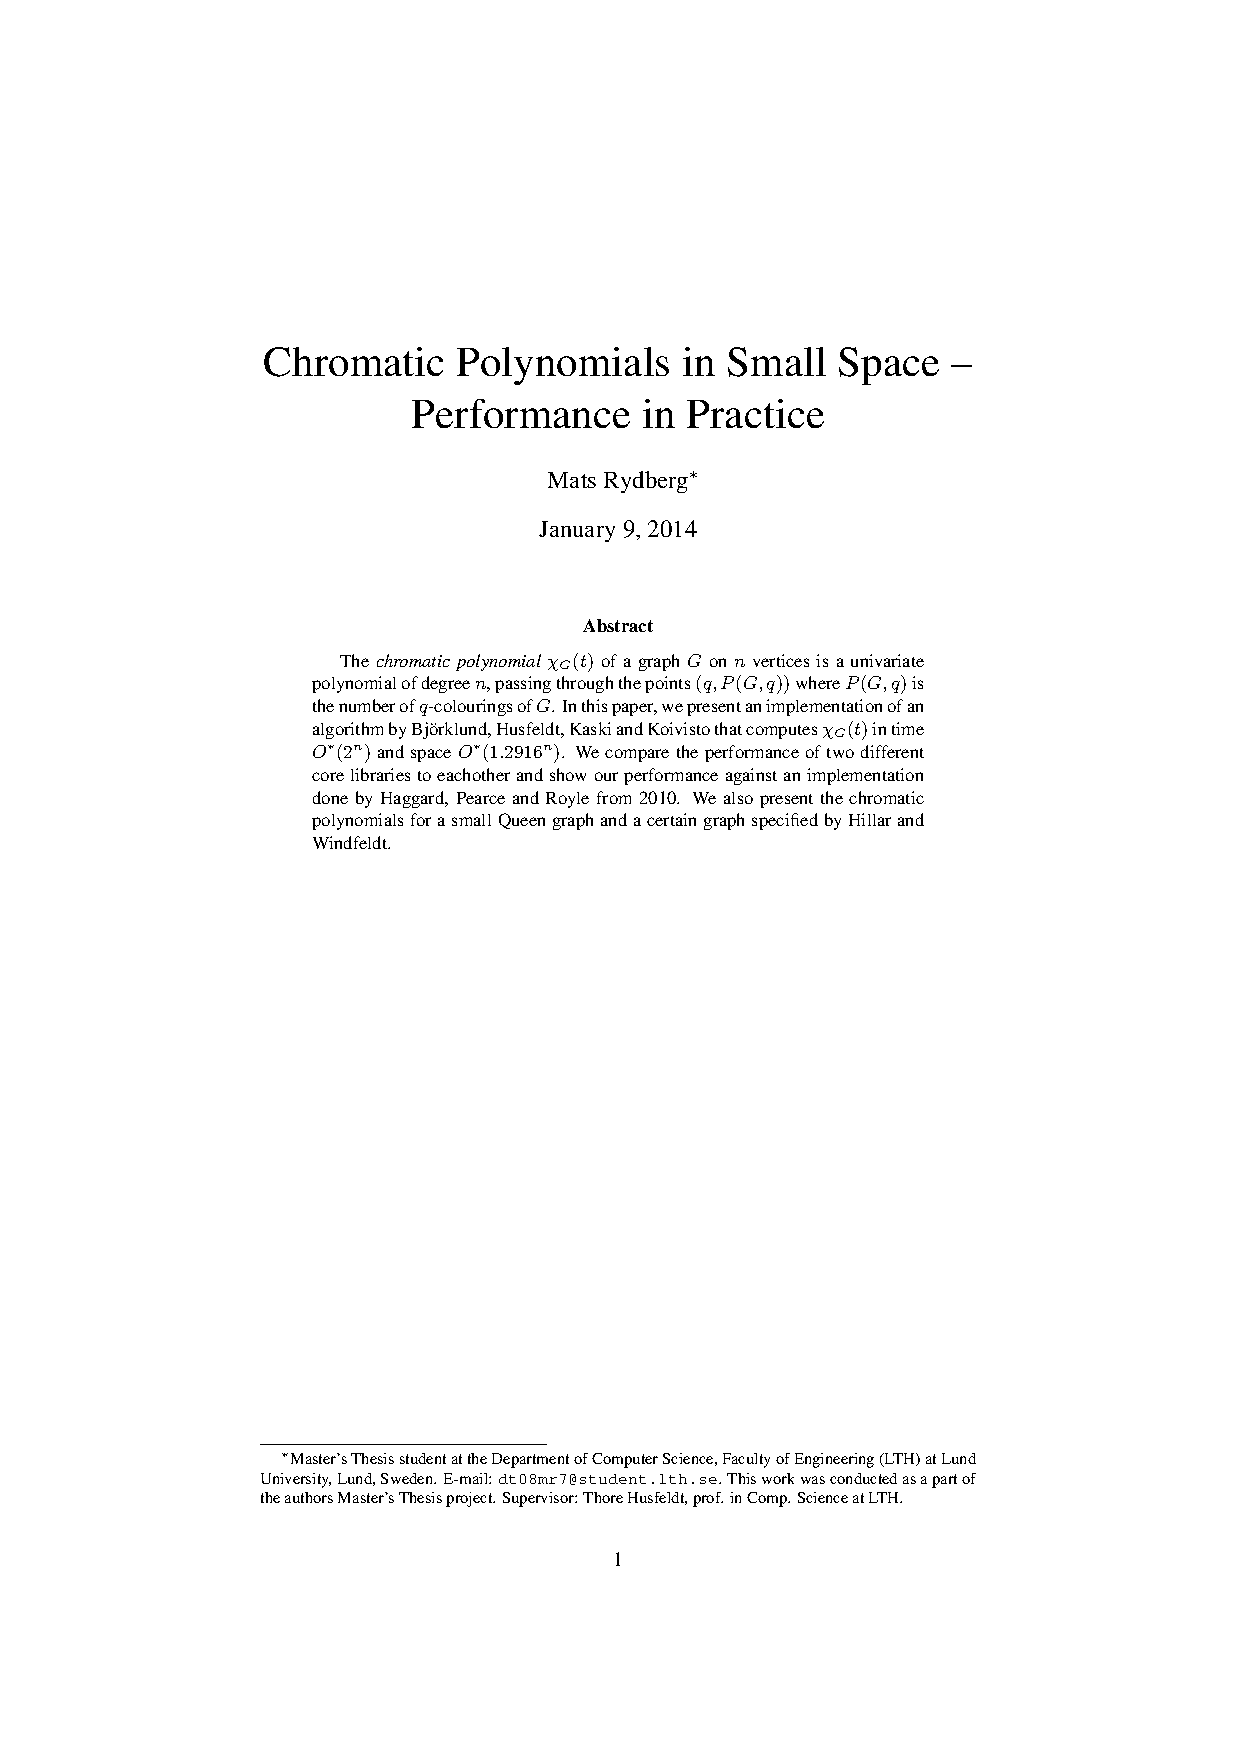
\includepdf[pages={-}]{12pages.pdf}
 
\end{appendices}


\end{document}
